\documentclass[paper=letter, fontsize=11pt]{scrartcl} 
\usepackage{graphicx}
\usepackage{verbatim}
\usepackage{pictex}  
\usepackage{multimedia}
\usepackage{listings}
\usepackage{xcolor,colortbl}
\usepackage[utf8]{inputenc}		%para identificar acentos(encoding)
\usepackage{url}
\usepackage[spanish]{babel} % language/hyphenation
\usepackage{amsmath,amsfonts,amsthm} % Math packages
\usepackage{amsbsy}
\usepackage{amssymb}
\usepackage{fancyvrb}
\usepackage{sectsty} % Allows customizing section commands
\allsectionsfont{\centering \normalfont\scshape} % Make all sections centered, the default font and small caps
\usepackage{float}%para fijar las figuras y tablas
\usepackage{placeins}%fija espacios
\usepackage{fancyhdr} % Custom headers and footers
\pagestyle{fancyplain} % Makes all pages in the document conform to the custom headers and footers
\fancyhead{} % No page header - if you want one, create it in the same way as the footers below
\fancyfoot[L]{} % Empty left footer
\fancyfoot[C]{} % Empty center footer
\fancyfoot[R]{\thepage} % Page numbering for right footer
\renewcommand{\headrulewidth}{0pt} % Remove header underlines
\renewcommand{\footrulewidth}{0pt} % Remove footer underlines
\setlength{\headheight}{13.6pt} % Customize the height of the header

\numberwithin{equation}{section} % Number equations within sections (i.e. 1.1, 1.2, 2.1, 2.2 instead of 1, 2, 3, 4)
\numberwithin{figure}{section} % Number figures within sections (i.e. 1.1, 1.2, 2.1, 2.2 instead of 1, 2, 3, 4)
\numberwithin{table}{section} % Number tables within sections (i.e. 1.1, 1.2, 2.1, 2.2 instead of 1, 2, 3, 4)

\setlength\parindent{0pt} % Removes all indentation from paragraphs - comment this line for an assignment with lots of text

\newcommand{\horrule}[1]{\rule{\linewidth}{#1}} % Create horizontal rule command with 1 argument of height

\title{	
\normalfont \normalsize 
\textsc{Centro de Investigaci\'on en Matem\'aticas (CIMAT). Unidad Monterrey} 
\\ [25pt] 
\horrule{0.5pt} \\[0.4cm] % Thin top horizontal rule
\huge Ciencia de datos (Tarea 3) \\ 
\horrule{2pt} \\[0.5cm] % Thick bottom horizontal rule
}

\author{José Antonio Garcia Ramirez} % Your name

\date{\normalsize\today} % Today's date or a custom date

\begin{document}
\lstdefinestyle{customc}{
  belowcaptionskip=1\baselineskip,
  basicstyle=\footnotesize, 
  frame=lrtb,
  breaklines=true,
  %frame=L,
  %xleftmargin=\parindent,
  language=C,
  showstringspaces=false,
  basicstyle=\footnotesize\ttfamily,
  keywordstyle=\bfseries\color{green!40!black},
  commentstyle=\itshape\color{red!40!black},
  identifierstyle=\color{blue},
  stringstyle=\color{purple},
}

\lstset{breakatwhitespace=true,
  basicstyle=\footnotesize, 
  commentstyle=\color{green},
  keywordstyle=\color{blue},
  stringstyle=\color{purple},
  language=C++,
  columns=fullflexible,
  keepspaces=true,
  breaklines=true,
  tabsize=3, 
  showstringspaces=false,
  extendedchars=true}

\lstset{ %
  language=R,    
  basicstyle=\footnotesize, 
  numbers=left,             
  numberstyle=\tiny\color{gray}, 
  stepnumber=1,              
  numbersep=5pt,             
  backgroundcolor=\color{white},
  showspaces=false,             
  showstringspaces=false,       
  showtabs=false,               
  frame=single,                 
  rulecolor=\color{black},      
  tabsize=2,                  
  captionpos=b,               
  breaklines=true,            
  breakatwhitespace=false,    
  title=\lstname,             
  keywordstyle=\color{blue},  
  commentstyle=\color{dkgreen},
  stringstyle=\color{mauve},   
  morekeywords={\%*\%,...}         
} 


\maketitle % Print the title

\section{Ejercicio 1}

\textit{Este ejercicio es sobre la evaluacion de diferentes algoritmos de clasicación binaria.}\\
\textit{Tenemos un conjunto de prueba y un conjunto de entrenamiento y dos algoritmos de clasicación $C_1$ y $C_2$ obtenidos con el mismo conjunto de entrenamiento. Define $X_i$ como la variable que indica si el algoritmo $C_i$ clasifica un dato del conjunto de prueba como 0 o 1 y define $Y_i$ como la variable que indica si el algoritmo $C_i$ lo clasifica correctamente o no. Lo anterior nos da dos tablas de contingencia (una basada en $(X_1,X_2)$ y otra en $(Y_1, Y_2)$).}\\
\begin{enumerate}
\item \textit{Una manera para cuanticar si los clasicadores se comportan de manera similar es vericar si las distribuciones marginales de $Y_i$ son iguales. Muestra que lo anterior es equivalente a vericar si $p_{0,1} = p_{1,0}$ con $p$ las probabilidades subyacentes a la tabla de contingencia de $(Y_1, Y_2)$. Deriva el estimador de Máxima Verosimilitud para esta hipótesis. Usa un estadístico de prueba basado en razones de verosimilitud para calcular el p-valor bajo esta hipótesis para los siguientes datos:}\\
\begin{table}[h]
\begin{center}
\begin{tabular}{c|cc}
\hline
    & $Y_2=0$ & $Y_2=1$\\\hline
$Y_1=0$ & 8& 7\\
$Y_1=1$ & 11 & 21\\\hline
\end{tabular}
\end{center}
\end{table}
\FloatBarrier
$ \longleftrightarrow $\\
Partamos del supuesto de que las marginales son iguales i.e. $P(Y_1)=P(Y_2)$\\
Queremos demostrar que $p_{0,1} = p_{1,0}$\\
Por definición:
\begin{equation}
\begin{split}
p_{0,1}=&P(Y_1=0,Y_2=1)=P(Y_1=0)P(Y_2=1)\\
      =&  (1- P(Y_1=1))(1- P(Y_2=0))\\
      =& 1-P(Y_2=0)-P(Y_1=1)+P(Y_2=0)P(Y_1=1)\\
      =& 1-P(Y_2=0)-P(Y_1=1) +P(Y_1=1,Y_2=0)\\
            =& 1-P(Y_2=0)-P(Y_1=1) +p_{1,0}\\
\end{split}
\end{equation}
Con lo anterior basta probar que $1-P(Y_2=0)-P(Y_1=1)$ vale cero, para ello recordemos que por la hipótesis que tenemos sobre las marginales $P(Y_1)=P(Y_2)$ implica que $P(Y_1=1)=P(Y_2=1)$ y que sus complementos también son iguales por lo que $P(Y_1=0)=P(Y_2=0)$.\\
Entonces:\\
\begin{equation*}
\begin{split}
1-P(Y_2=0)-P(Y_1=1) &= (P(Y_1 = 1)+P(Y_1=0)) + P(Y_1=0) -P(Y_2=0)-P(Y_1=1)\\
&= P(Y_1=0)-P(Y_2=0) = 0
\end{split}
\end{equation*}
Entonces la última igualdad en (1.1) queda como \[p_{0,1}= 1-P(Y_2=0)-P(Y_1=1) +p_{1,0} = 0+p_{1,0}\]

%\begin{figure}[H]
 % \begin{center}
%    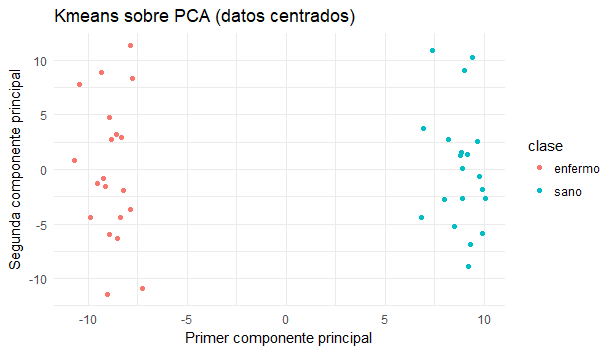
\includegraphics[scale=.75]{kmeans_genes_pca.png}
  %  \caption{Resultado promedio de k-means sobre el conjunto de datos escalado, proyectado en las dos primeras componentes, considerando PCA con una matriz de correlación.}
   % \label{figura1_1}
  %\end{center}
%\end{figure}


 Entonces estamos tratando con una distribución multinomial v.a. porque cada una de las $n$ observaciones cae en una de las 4 casillas de la tabla de contingencia. De nuestro curso de inferencia estadística sabemos que la expresión de la v.a. binomial es $\frac{n!}{x_1!x_2!}p_1^{x_1}p_2^{x_2}$ (en el caso de dos categorías).\\
 Y como la distribución multinomial comparte propiedades con la Binomial, sabemos que el estimador de máxima verosimilitud de $p$ esta dado por $p_{ML}= n p_{i+}p_{+j}$ donde $p_{i+}$ y $p_{+j}$ son las proporciones de los casos favorables por filas y reglones respectivamente, así  $p_{ML}= n (\frac{n_{i+}}{n} ) (\frac{n_{+j}}{n} ) = \frac{n_{i+}n_{+j}}{n} $
 Entonces en nuestra hipótesis nula correspondiente a la independencia de los clasificadores (despues de un poco de algebra) se reduce a que el numerador es de la forma $n_{ij}$ el numero de casos observados en la casilla $(i,j)$ de la tabla de contingencia, dividido por el estimador maximoverosimiles acabamos de deducir y este cociente se eleva a la potencia $n_{ij}$, recordando que tenemos $i$ fila y $j$ entradas y que el logaritmo de un producto es la suma de los logaritmos tenemos que el radio de verosimilitud esta dado por :
\[
2\sum_{i,j}n_{ij}(n_{ij})\ln\left(\frac{n_ij}{p_{ML}} \right)
\]
Y como tambien vimos que para muestras grandes la prueba de máxima verosimilitud es uniformemente más potente para la familia exponencial y que para muestras grande converge en distribución a la $\chi^2$ (en nuestro caso con un grado de libertad), podemos realizar el calculo por lo que nuestro estadístico de prueba es $G=1.51$ y el p-value es $p-value=1-\chi^2_1(1.51)\approx0.22$ por lo que no rechazamos la hipotesis de independcia lo que implica que los clasificadores son "igual de buenos".


\item \textit{¿Qué complicaciones habría al utilizar las $X$'s en lugar de las $Y$'s?}\\
Pues la prueba de hipótesis se complica, debido a que tendríamos que considerar la distribución conjunta de $(X_1,X_2)$ lo cual a pesar de que las $X$'s son independientes es el producto de dos distribuciones binomiales, donde además los parámetros varían, y aumenta la dimensión en la estimación maximoverosimil para el denominador de la prueba. 
\end{enumerate}



\section{Ejercicio 2}
\textit{Para datos de clasicacion binaria $\{(x_i, y_i)\}_{i=1}^n$ considera la siguiente función de costo:}
\begin{equation}
L = \sum_{i}(\theta(y_i)-\beta^tx_i-\beta_0)^2
\end{equation}
\textit{Denimos $n_+,n_-$ el número de observaciones con $y_i = 1$ y $y_i = -1$, respectvamente $c_+, c_-$ el centroide de las observaciones con $y_i = 1$ y $y_i = -1$ y $c$ el centroide de todos los datos.\\
Como en clase, construimos las matrices:}
\[
S_B = (c_+ - c_-)(c_+ - c_-)^t
\]
\[
S_W = \sum_{i:y_i=1}(x_i - c_+)(x_i - c_+)^t + \sum_{i:y_i=-1}(x_i - c_-)(x_i - c_-)^t
\]
\begin{enumerate}
\item\textit{ Verifica que }\\
\[
S_W=\sum_{i:y_i=1}x_ix_i^t+\sum_{i:y_i=-1}x_ix_i^t-n_+c_+c_+^t-n_-c_-c_-^t
\]
Lo verificamos:\\

\begin{equation*}
\begin{split}
S_W &= \sum_{i:y_i=1}(x_i - c_+)(x_i - c_+)^t + \sum_{i:y_i=-1}(x_i - c_-)(x_i - c_-)^t\\
= & \sum_{i:y_i=1}(x_i - c_+)(x_i^t - c_+^t) + \sum_{i:y_i=-1}(x_i - c_-)(x_i^t - c_-^t)\\
= & \sum_{i:y_i=1}(x_ix_i^t- x_ic_+^t - c_+x_i^t + c_+c_+^t) + \sum_{i:y_i=-1}(x_ix_i^t- x_ic_-^t - c_-^tx_i^t + c_-c_-^t)\\
= & (\sum_{i:y_i=1}x_ix_i^t + \sum_{i:y_i=-1}x_ix_i^t) - \sum_{i:y_i=1}(x_ic_+^t + c_+x_i^t) + \sum_{i:y_i=1}(c_+c_+^t)  -\sum_{i:y_i=-1}( x_ic_-^t+ c_-x_i^t) + \sum_{i:y_i=-1}(c_-c_-^t)\\
= & \sum_{i:y_i=1}x_ix_i^t + \sum_{i:y_i=-1}x_ix_i^t - \sum_{i:y_i=1}(x_ic_+^t + (x_ic_-^t)^t) + n_+(c_+c_+^t)  -\sum_{i:y_i=-1}( x_ic_-^t+ (x_ic_-^t)^t) + n_-(c_-c_-^t)\\
= & \sum_{i:y_i=1}x_ix_i^t + \sum_{i:y_i=-1}x_ix_i^t - \sum_{i:y_i=1}x_ic_+^t - \sum_{i:y_i=1}(x_ic_+^t)^t + n_+(c_+c_+^t) \\
-& \sum_{i:y_i=-1}x_ic_-^t - \sum_{i:y_i=-1}(x_ic_-^t)^t + n_-(c_-c_-^t) \\
= & \sum_{i:y_i=1}x_ix_i^t - \sum_{i:y_i=-1}x_ix_i^t - n_+c_+c_+^t - n_+(c_+c_+^t)^t + n_+(c_+c_+^t) 
- n_-c_-c_-^t - n_-(c_-c_-^t)^t + n_-(c_-c_-^t) \\
= & \sum_{i:y_i=1}x_ix_i^t - \sum_{i:y_i=-1}x_ix_i^t  - n_+(c_+c_+^t)^t - n_-(c_-c_-^t)^t  \\
\end{split}
\end{equation*}

Y como las matricez $(c_+c_+^t)^t$ y $(c_-c_-^t)^t$ son simétricas tenemos el resultado.
\item \textit{Verifíca que el vector $S_B\beta$, es un multiplo del vector $(c_+ - c_-)$, i.e. $S_B\beta = \lambda (c_+ - c_-)$}\\

Observemos que el producto $S_B\beta$ lo pdodemos ver de la siguiente manera: $S_B \beta = (c_+-c_-)\left((c_+-c_-)^t\beta \right )$, entonces el producto que es encuentra entre paréntesis es un producto punto que forma el coeficiente $\lambda$ del ejercicio.

\item \textit{Si definimos $\theta(1) = n/n_+$ y $\theta (-1) = n/n_-$, verica que en el mnimo de (2.1) es:}
\begin{equation*}
\beta_0=-\beta^tc
\end{equation*}
\begin{equation}
(S_W+\frac{n_+n_-}{n}S_B)\beta=n(c_+-c_-)
\end{equation}
Comenzamos con $\beta_0$, despues de derivar la función de costo con respecto a $\beta_0$ e igualar  cero obtenemos:

\begin{equation*}
\begin{split}
0 & =  \sum_i (\theta(y_i)- \beta^tx_i-\beta_0) \\
 & =  \sum_i\theta(y_i) - \sum_i\beta_0 -\sum_i\beta\\
 & = \sum_{i:y_i=1}\theta(y_i) + \sum_{i:y_i=-1}\theta(y_i) - \sum_i\beta_0 -\sum_i\beta\\
 & = (n_+ \frac{n}{n_+}) - (n_- \frac{n}{n_-}) - \sum_i\beta_0 - \sum_i\beta^t x_i \\
 & = -n\beta_0 - \beta^t \sum_ix_i +n -n\\
 &= -n\beta_0 - \beta^tcn\\
 & = \beta_0 +\beta^tc \\
\Rightarrow  & \beta_0= -\beta^tc  \\
\end{split}
\end{equation*}
Para la siguiente parte, de manera análoga derivamos la función de costo con respecto a $\beta$ e igualando a cero, usando el resultado anterior en la cuarta igualdad: 
\begin{equation*}
\begin{split}
0 & =  \sum_i (\theta(y_i)- \beta^tx_i-\beta_0)x_i^t \\
 & =  \sum_i\theta(y_i)x_i^t - \sum_i\beta_0x_i^t -\sum_i\beta x_ix_i^t\\
 & = \sum_{i:y_i=1}\theta(y_i)x_i^t + \sum_{i:y_i=-1}\theta(y_i)x_i^t - \beta_0\sum_ix_i^t -\beta \sum_ix_ix_i^t\\
 & = (n \frac{\sum_{i:y=1} x_i}{n_+}) - (n \frac{\sum_{i:y=-1}x_i}{n_-}) - (-\beta^tc)\sum_ix_i^t - \beta^t\sum_ix_i x_i^t \\
 & = nc_+ - nc_- - \beta^t( \sum_ix_ix_i^t-c\sum^t_ix_i^t) \\
 \Rightarrow & \beta^t( \sum_ix_ix_i^t-c\sum_ix_i^t) = n(c_+-c_-)\\
 \Longleftrightarrow &  \beta^t( S_W +n_+ c_+c_+^t +n_-c_-c_-^t -ncc^t ) = n(c_+-c_-) \\
\end{split}
\end{equation*}
Por un lado, tenemos que 
\[  nc = \sum_i x_i = \sum_{i:y=1}x_i +\sum_{i:y=-1}x_i = n_+c_+ + n_-c_- \]
Así que si lo aplicamos a la anterior igualdad tenemos:

\begin{equation*}
\begin{split}
n(c_+-c_-) = & \beta ^t( S_W + n_+ c_+ c_+^t + n_-c_-c_-^t -n c c^t ) \\
= & \beta^t( S_W +n_+ c_+c_+^t +n_-c_-c_-^t -(n_+c_+ + n_-c_-)c^t ) \\
= & \beta^t( S_W +n_+ c_+c_+^t +n_-c_-c_-^t -\frac{n_+c_+ + n_-c_-}{n}(n_+c_+^t+n_-c_-^t ) )\\
= & \beta^t( S_W +n_+ c_+c_+^t +n_-c_-c_-^t -\frac{n_+^2c_+c_+^t +n_+c_+n_-c_-^t + n_-c_-n_+c_+^t + n_-^2c_-c_-^t }{n}) \\
= & \beta^t( S_W + \frac{c_+c_+^tn_+(n-n_+) +n_-c_-c_-^t(n-n_-)+ n_+n_-c_+c_-+n_+n_-c_-c_+)}{n} )  \\
= & \beta^t( S_W + \frac{c_+c_+^tn_+(n_-) +n_-c_-c_-^t(n_+)+ n_+n_-c_+ c_-^t + n_+n_-c_-c_+^t)}{n} \\
= & \beta^t( S_W + \frac{n_+n_-(c_+c_+^t+c_-c_-^t+ c_+c_-^t +c_-c_+^t)}{n}) \\
\end{split}
\end{equation*}

Y al realizar el primer ejercicio encontramos que $S_B = c_+c_+^t -c_+c_-^t -c_1c_+^t + c_- c_-^t $ y conectándolo con la igualdad anterior tenemos y transponiendo tenemos el resultado. Pues las matrices $S_B$ y $S_W$ son simétricas. 


\item \textit{Usando el resultado de inciso b, argumenta que (2.2) implica que en el mínimo:}
\[\beta \sim S_x^{-1}(c_+-c_-) \]
\textit{Es decir que la solución coincide con la del Fisher Discriminant Analysis (FDA).}

Como en el segundo inciso de este ejercicio supongamos que sin pérdida de generalidad que $S_B \beta= \lambda (c_+-c_-)$ en vista de que el lado derecho es un múltiplo del lado izquierdo, con $\lambda$ un escalar.

Tenemos los siguiente primero realizamos el producto del inciso anterior y lo siguiente solo es algebra:

\begin{equation*}
\begin{split}
(S_W+\frac{n_+n_-}{n}S_B)\beta = & n(c_+-c_-)\\
S_W\beta + \frac{n_+n_-}{n}\lambda(c_+-c_-) =& n(c_+-c_-)\\
\Longleftrightarrow  S_W\beta  = &  n(c_+-c_-)- \frac{n_+n_-}{n} \lambda(c_+-c_-)\\
\Longleftrightarrow  \beta  = &  S_W^{-1}(c_+-c_-)(n- \frac{n_+n_-\lambda}{n} )\\
\end{split}
\end{equation*}
De donde $\beta \approx  S_W^{-1}(c_+-c_-)$


\item \textit{Lo anterior permite implementar FDA usando algún algoritmo de mínimos cuadrados.
En R lo haremos con la funcion lm(). Ilustra cómo funciona el método con algunos conjuntos de datos en 2D bien elegidos.}

La implementación que realicé se anexa en el archivo ‘ejercicio2.R’, En la figura 2.1 se encuentra dos ejemplos que construí es importante mencionar que, aunque por construcción ambas muestras son linealmente separables el coeficiente $\beta$ estimado de la manera que pide el ejercicio es una aproximación al separador lineal óptimo por que se observan varios errores de clasificación. La primer muestra en la figura 2.1 (arriba) fue generada con dos v.a. con distribución $Exp(1)$ mientras que la otra se generó con dos distribuciones $Unif(0,1)$ en ambos casos la separación se efectuó con la recta identidad. Notemos que en ambas simulaciones existen varios datos atípicos lejos de los centroides.
 


\begin{figure}[H]
  \begin{center}
    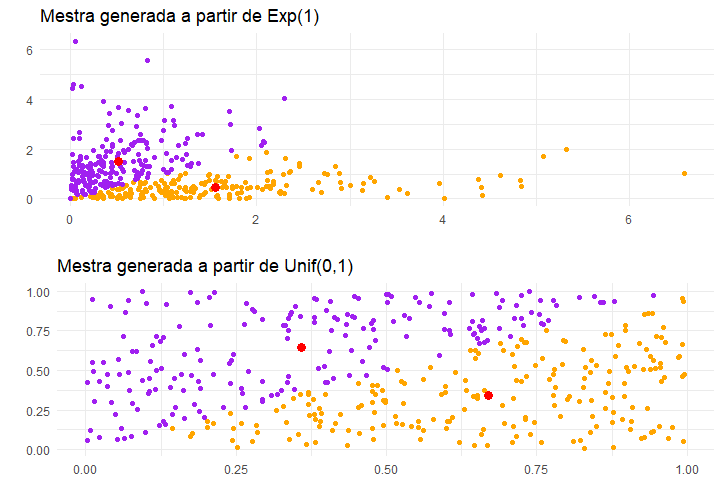
\includegraphics[scale=.7]{aprox_lda_unif.png}
    \caption{Muestras de tamaño 400 generadas con una distribución uniforme en [0,1] (abajo) y exponencial (arriba) con parámetro $\lambda = 1$, las categorías fueron asignadas si la observación se encuentra por debajo o por arriba de la identidad. Los punto en rojo corresponden a los centroides de cada grupo. En ambos casos la presición de clasificación fue mayor al 97\%.  }
    \label{figura2_1}
  \end{center}
\end{figure}
\FloatBarrier


\item \textit{Observamos que (2.1) muestra que FDA \textbf{no} es muy robusto a datos atípicos.\\
Una posibilidad para hacerlo más robusto es usar mínimos cuadrados ponderados. Por
ejemplo lm() tiene un argumento opcional weights donde se pueden proporcionar pesos $w_i,i = 1,..., n$ para minimizar:}
\[
\sum_i w_i (\theta(y_i)-\beta^tx_i-\beta_0)^2
\]
\textit{¿Cómo elegirías estos pesos? ¿Verifica tu propuesta con algunos ejemplos en 2D.}
\end{enumerate}
Una posible elección que considere para los pesos $w_i$ de las observaciones fue el de asignarlos a la distancia de Mahalanobis (considerando cada categoría por separado), otra opción que probé fue la de asignar los inversos multiplicativos de estos pesos, puede ser que debido al rango de los datos esta diferencia no se tan marcada. Con una inspección visual considere que usar los inversos multiplicativos de los pesos de las distancias de Mahalanobis se desempeña ligeramente mejor.

\begin{figure}[H]
  \begin{center}
    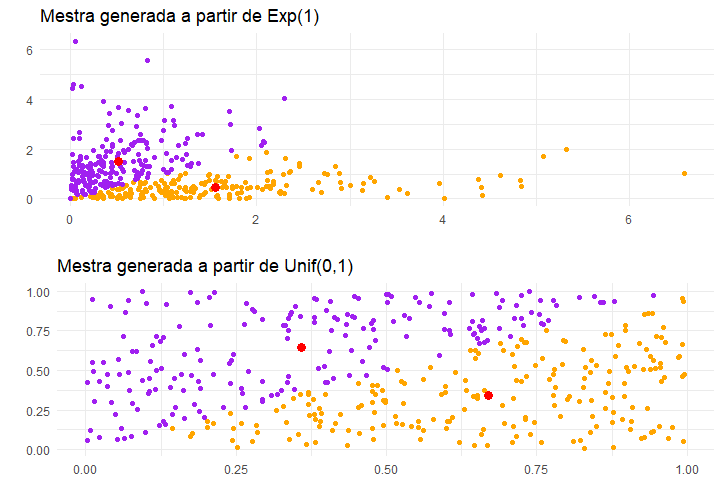
\includegraphics[scale=.8]{figura2_2.png}
    \caption{ Las mismas muestras generadas en la figura 2.1, sin embargo, en esta  gráfica la estimación del separador lineal se efectuó considerando pesos para las poblaciones. En ambos casos se logró una precisión de clasificación mayor al 98\% }
    \label{figura2_2}
  \end{center}
\end{figure}
\FloatBarrier

\section{Ejercicio 3}
\textit{Este ejercicio es sobre el método de clasicacion binaria perceptrón.}

\begin{enumerate}
\item \textit{Implementa el modelo clásico de perceptrón (version que trabaja en línea). Aplícalo
primero a un conjunto de datos articiales en dos dimensiones y con dos categorias.\\
Discute tus resultados. Incluye gráficas del ajuste.}\\

En vista de que estamos clasificando consideré la implementación sencilla vista en clase, que considera la función de perdida dada por:
 
\[
L(\beta) = -\sum_{i=1}^n \sum_{k=1}^ny_{ik}\ln( \hat{y}_{ik}) 
\]


La implementación la anexo en el archivo ‘ejercicio3.R’, para probarla generé dos grupos de muestras normal bivariada (en el codigo se encuentran los detalles de la muestra), de tamaño 1000 cada grupo.

Es importante mencionar que siguiendo las sugerencias del texto \cite{Hes} los datos se escalaron (se restó la media y se dividió por la desviación estándar) para tener mayor precisión en los cálculos numéricos, el vector de pesos se inicializó con valores cercanos a cero con una distribución $Unif(-0.7,0.7)$ siguiendo la sugerencia de \cite{Hes}. \\
En promedio el accuracy de la implementación con los parámetros fijos se encuentra en el rango [ 0.75, 0.96].
\begin{figure}[H]
  \begin{center}
    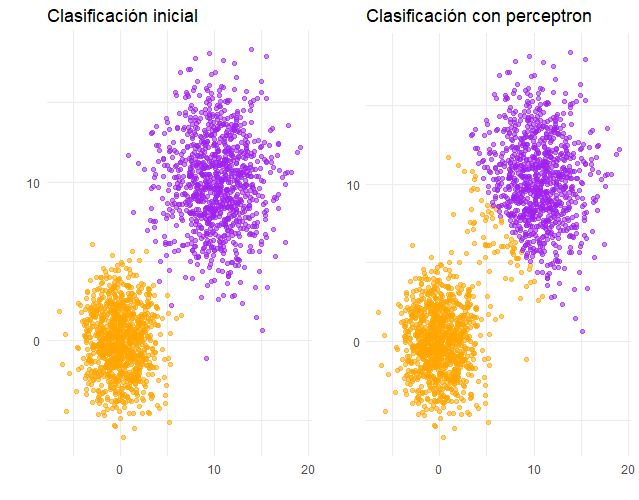
\includegraphics[scale=.7]{perceptron.png}
    \caption{ Clasificación efectuada por la implementación del perceptrón (izquierda) clasificación original y (derecha) clasificación efectuada fijando los parámetros de máxima numero de iteraciones a 6000.}
    \label{figura2_3}
  \end{center}
\end{figure}

Lo cual es malo, porque aunque la muestra se genera constantemente provienen de la misma distribución y en la figura 3.1 es fácil notar que los conjuntos son casi linealmente separables.

 
\item \textit{Aplica el clasicador al conjunto de datos \textbf{pima} que vimos en clase. Usa \textbf{pima.tr} para ajustar el modelo y \textbf{pima.te} para vericar su calidad predictiva. ¿ Qué puedes decir sobre su desempeño? Comenta tus hallazgos.}\\

Esta fue una gran oportunidad, personalmente, trabajar de nuevo con este conjunto de datos para no cometer de nuevo los errores que cometí hace unos años (ver \url{ https://www.overleaf.com/read/bshhzyjwcjps}) . Se agradece el preprocesamiento que realizaron mis profesores con el preprocesamiento del dataset, pues en una primer vista ya no existen ceros en las variables (esto en su momento fue un detalle pues la documentación del dataset decía que los nulos se reportaron como cero). Tambien es curioso la historia de este dataset que dista de los 70 aprox. Primero porque se popularizo y posteriormente dejo de estar en los repositorios de UCI y ahora está en Kaggle junto con un bonito diccionario de datos \url{ https://www.kaggle.com/uciml/pima-indians-diabetes-database/data} . Como comentario final y personal la variable que mide el Índice de peligre tienen una historia interesante, aunque es dificil de rastrear la fuente original, es esencialmente un promedio ponderado del número de personas diabéticas de las mujeres sujetas de estudio.\\

Para el conjunto de datos de los indios Pima, con que el que se trabaja en este ejercicio, al fijar la tasa de aprendizaje a $0.01$ y variar el número de iteraciones por 3 veces el numero de registros en el conjunto de entrenamiento se lograban un accuracy en el rango de $[0.33, 0.55]$ para ambos conjuntos prueba, por otro lado al fijar la misma tasa y descender el número de iteraciones a 200 se logró un accuracy en el rango de $[.6,0.7]$ mismo que es superior a lo que encontré en el trabajo al que hice referencia en el primer párrafo. La lección aprendida de este ejercicio es no olvidar que la estimación del perceptrón depende fuertemente de los parámetros mencionados y del punto de inicio (que en este caso dejamos fijo también). En la figura 3.2 podemos apreciar una visualización de los datos de test, a la izquierda la clasificación original y a la derecha la clasificación del perceptrón que implementamos.
    

\begin{figure}[H]
  \begin{center}
    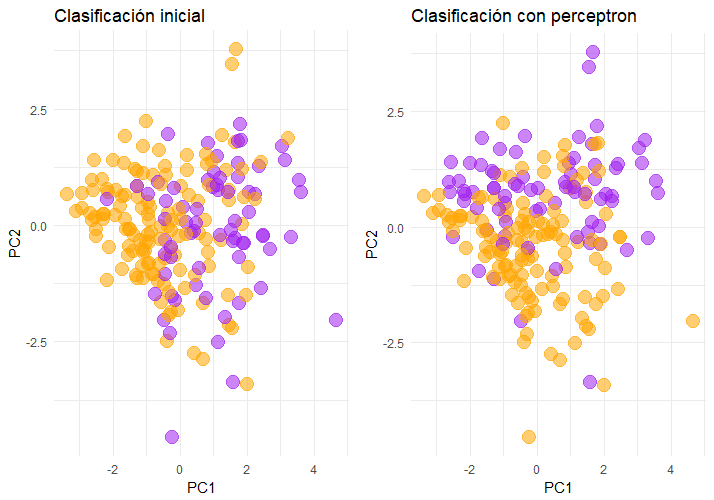
\includegraphics[scale=.65]{pima.png}
    \caption{ Proyección en componentes principales, usando la matriz de correlacion, de los datos de test. (Derecha) clasificación del perceptrón y (izquierda) clasificación autentica. Los puntos en amarillo corresponden a mujeres sin diabetes, los puntos en morado indican que la prueba de diabetes fue positiva.}
    \label{figura3_2}
  \end{center}
\end{figure}
\FloatBarrier

\end{enumerate}


\section{Ejercicio 4}
\textit{Implementa Kernel FDA. Puedes basarte en el artculo de Mika et al: \textbf{Fisher Discriminant Analysis with kernels}. Verica su desempeño en un conjunto de datos articiales apropiados en dos dimensiones y dos clases. Compara su desempe~no con FDA estandar en el conjunto de datos pima del ejercicio 3b. Comenta tus hallazgos.}\\

Basándome en el paper mencionado mi implementación se base en la redacción del texto, la parte esencial se encuentre en construir las matrices $N$ y $M$ que define el trabajo mencionado. La implementación es en R pero se utilizaron herramientas del package ‘Rcpp’ para construir de manera rápida las matrices de Kernel además del uso del package ‘RSpectra’ para obtener el vector propio asociado al valor propio más grande de la matriz $N^{-1}M$, que es una interfaz a la librería Spectra que es una reconstrucción de la clásica librería LAPACK pero desarrollada en Fortran. En la implementación se siguió la idea del paper acerca de forzar a que $N$ sea definida positiva, lo cual aumenta un parámetro (experimentalmente encontramos que es conveniente que este valor $\mu$ sea pequeño).La actual implementación solo utiliza un kernel gaussiano de la forma $e^{-||x_i-x_j||^2_2/\sigma}$. El código de mi implementación en se incluye en el archivo ‘ejercicio4general.r’ al igual que el archivo ‘KernelLDA.cpp’.\\

Para comenzar genere una muestra la cual consiste en 400 observaciones de las cuales las 200 primeras corresponden a una circunferencia con centro en $(0.5,0 .5)^t$ y de radio 1 a las cuales en cada componente agregue ruido con distribución N(0,1/10), las segundas 200 observaciones corresponden a una circunferencia con el mismo centro pero con radio 4, también en cada componente se agregó ruido con la misma distribución, posteriormente escale los datos. En la figura 4.2 se muestra la muestra aleatoria generada y su clasificación original.\\  
En vista de que el tiempo de ejecución de la implementación de KLDA que realice es prudente para muestras de tamaño pequeño (aquí es importante mencionar que la complejidad de los métodos de kernel radica en el número de observaciones, si bien el número de variables aporta menos en la complejidad en tiempo no debemos olvidar que eso conlleva a la maldición de la dimensionalidad), me permitió realizar una búsqueda en el espació de parámetros para ambos conjuntos de datos. En la figura 4.1 podemos apreciar en el eje ‘x’ el accuracy del algoritmo en el conjunto de entrenamiento, análogamente en el eje ‘y’ se encuentra el accuracy obtenido sobre el conjunto de prueba, la búsqueda de los parámetros se realizó sobre un grid igualmente espaciado, cuadrado y con un total de 10,000 puntos, donde  $\mu \in [0.32, 7]$ mientras que $\sigma \in [35, 100]$.   \\

El tiempo de ejecución de la búsqueda fue de aproximadamente 6 mins (en un ambiente Windows no multicore), como podemos ver en la grafica 4.1, parece haber estabilidad en los parámetros pues al notar que el tamaño del punto (cuyas coordenadas representan a la precisión de entrenamiento y de validación del algoritmo) corresponde al valor $\sigma$ mientras que la intensidad del color azul permite visualizar el valor de $\mu$. Decidimos ser conservadores y tomar el punto $(0.8, 0.84 )$ que tiene asociados los valores “buenos” de los parámetros (considerando que es una muestra simulada) por lo que $\mu = 7$ y $\sigma=100$.

\begin{figure}[H]
  \begin{center}
    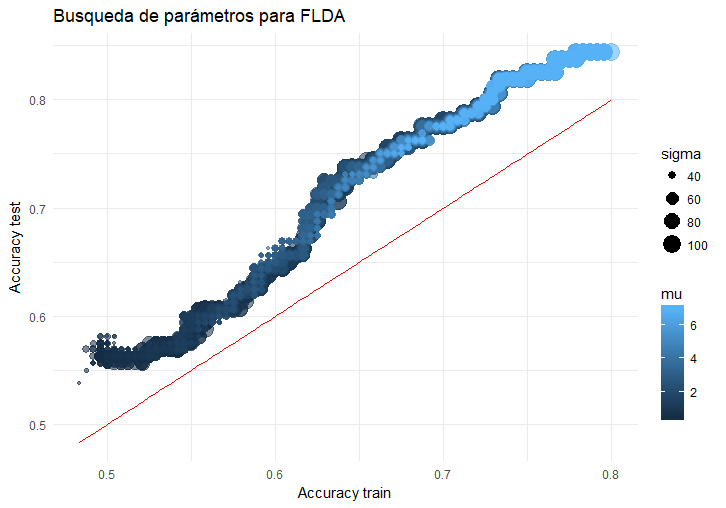
\includegraphics[scale=0.65]{grid_donas.png}
    \caption{Precisión obtenida en el conjunto de entrenamiento vs la obtenida en el conjunto de prueba en la muestra simualda, el tamaño de los puntos indica el valor del parámetro $\sigma$, el color el valor para $\mu$ y la recta en rojo es la identidad.   }
    \label{figura4_2}
  \end{center}
\end{figure}


Como podemos ver en la figura 4.2 la separación no se logró, pese a la búsqueda “extensiva” de los parámetros. Cabe mencionar que la submuestra con la que se entreno el algoritmo corresponde al 70\% de la muestra total. 

\begin{figure}[H]
  \begin{center}
    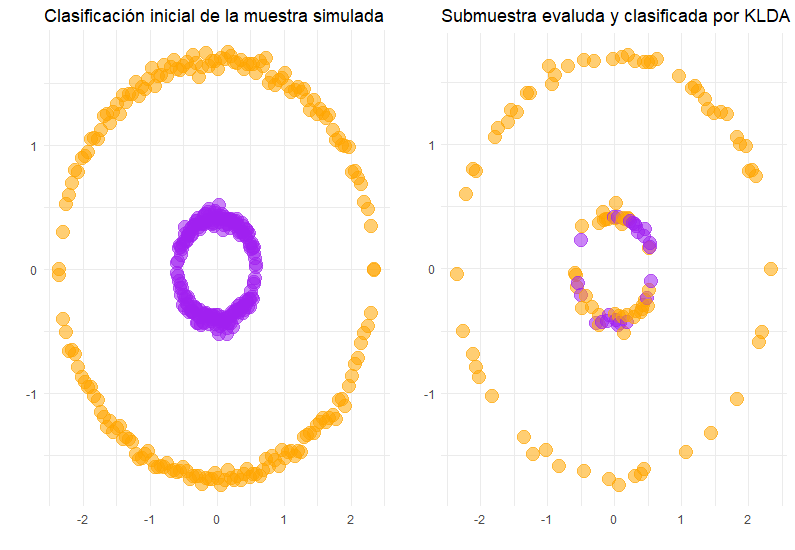
\includegraphics[scale=0.4]{donas_kernel.png}
    \caption{Conjunto de datos simulados inicialmente (izquierda) y la clasificación de la implementación de KLDA con parámetros $\mu = 7$ y $\sigma = 100$ (derecha)  }
    \label{figura4_2}
  \end{center}
\end{figure}

En cuanto a nuestro, ya familiar, conjunto de datos PIMA, el cual consiste en 332 observaciones para entrenamiento y 200 observaciones para validación, se procedió de manera análoga al conjunto de datos anterior (salvo la homologación de la variable respuesta) se realizó una búsqueda en el espació de parámetros. En la figura 4.3 podemos observar los accuracy obtenidos al variar los parámetros (con la misma convención de ejes, tamaño y color que la imagen 4.1), la búsqueda de los parámetros se realizó sobre un grid igualmente espaciado, cuadrado y con un total de  22,500 puntos, donde $\mu \in [0.0001, 7]$ mientras que $\sigma \in [0.0001, 150]$ (el tiempo de ejecución de la búsqueda fue de aproximadamente 1 hr y 40 mins).\\
En la figura 4.3 podemos ver que la sensibilidad en los parámetros es mayor en comparación al ejercicio pasado. Decidimos ser conservadores y tomar los valores del punto $(0.578, 0.575 )$ como los valores “buenos” de los parámetros así $\mu = 0.046$ y $\sigma=44.29$.

\begin{figure}[H]
  \begin{center}
    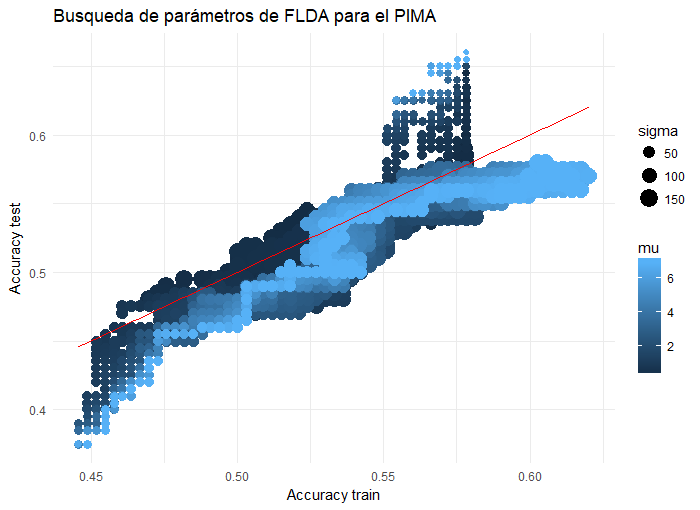
\includegraphics[scale=0.75]{grid_pimas.png}
    \caption{Precisión obtenida en el conjunto de entrenamiento vs la obtenida en el conjunto de prueba para el dataset PIMA, el tamaño de los puntos indica el valor del parámetro $\sigma$, el color el valor para $\mu$ y la recta en rojo es la identidad.   }
    \label{figura4_3}
  \end{center}
\end{figure}

Como podemos ver en la figura 4.4 la separación no se logró, pese a la búsqueda “extensiva” de los parámetros y aún teniendo muestras balanceadas pues en el conjunto train el 32.8\% de sus observaciones son positivas mientras que en el conjunto test el 34\% lo son.\\
En este punto queremos aclarar el termino ‘conservador’ al que nos hemos referido en la elección de los parámetros, por ejemplo en la figura 4.3 una opción greedy seria tomar los valores correspondientes al punto que se encuentra arriba a la derecha pero en esa imagen es fácil distinguir un conjunto de puntos que se encuentran en la parte superior, en ese ejemplo tomamos uno de esos puntos y como pudimos comprobar la separación no es perfecta; por otro lado el comportamiento de los puntos en el conjunto de datos PIMA (los pares de precisión en el conjunto de entrenamiento y en el de prueba) nos ilustran lo complicado que puede ser buscar parámetros “óptimos” despues de elegir un modelo. Y bien no olvidemos que estos resultados aplican para la partición que se nos dio, pues otra partición generaría un conjunto de puntos diferentes (aunque parecidos), es uno de los temas que tratamos en la última clase sobre la dimensión de Vapnik-Chervonenkis y ello me motivo a dedicarle tiempo a este ejercicio (que por cierto me agrado bastante).\\
En el archivo ‘searchParametrosKLD.R’ incluyo un pequeño codigo así como el archivo ‘w\_KLD.zip’ para compartir una gráfica interactiva y más informativa que la figura  4.3, anexo también el archivo 'visualizacion\_busqueda\_de\_parametros\_ejercicio\_4.html' que permite compartir la visualización interactiva que menciono.\\
En la figura 4.4 se muestran los resultados de la clasificación sobre el conjunto test de la implementación de KLDA.

\begin{figure}[H]
  \begin{center}
    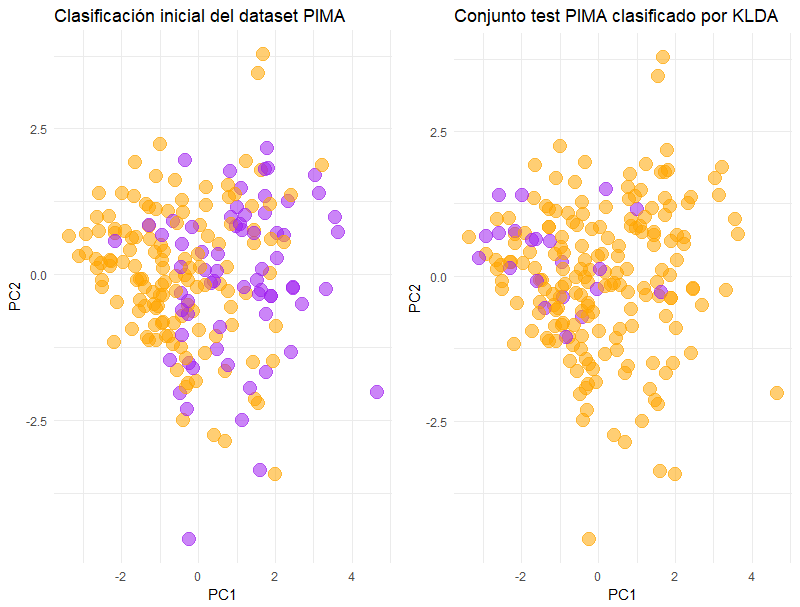
\includegraphics[scale=0.7]{kernel_pima.png}
    \caption{Proyeccion en las dos primeras componentes principales, usando matriz de correlación, del conjunto de datos PIMA con su etiqueta natural (izquierda) y la clasificación de la implementación de KLDA con parámetros $\mu = 1.97$ y $\sigma = 8.58$  con un accuracy en en conjunto train de 57\% y 62\% en el test. }
    \label{figura4_4}
  \end{center}
\end{figure}


 Finalmente, al comparar el desempeño sobre los dos conjuntos de datos, de nuestra implementación con kernels (y la exhaustiva búsqueda de parámetros) encontramos que la clasificación con LDA logra una precisión de 84\% en el conjunto de prueba, la clasificación efectuada por LDA se muestra en la figura 4.5 con esto concluimos que nuestra implementación tiene muchas áreas de oportunidad como usar otros kernels. 
\begin{figure}[H]
  \begin{center}
    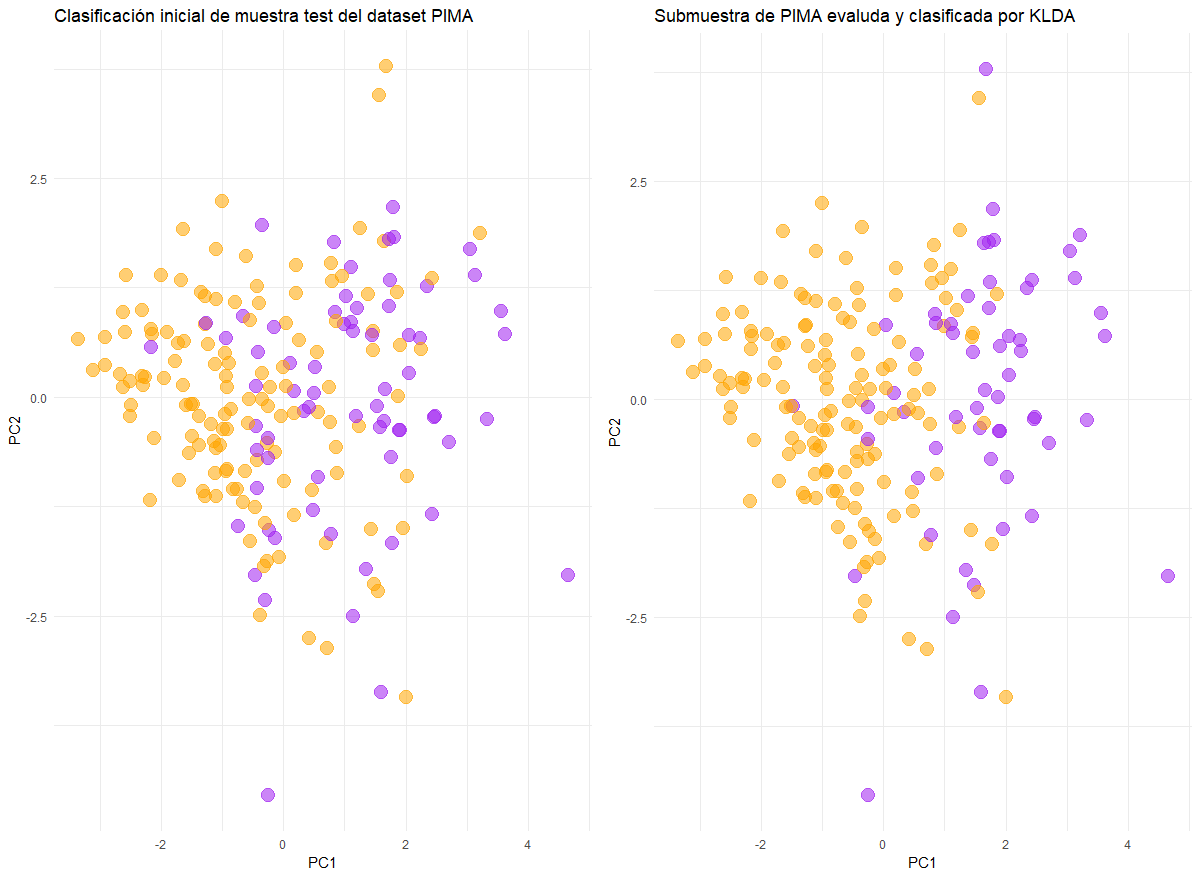
\includegraphics[scale=0.45]{lda_pima.png}
    \caption{Proyeccion en las dos primeras componentes principales, usando matriz de correlación, del conjunto de datos PIMA con su etiqueta natural (izquierda) y la clasificación de la implementación de LDA con parámetros con un accuracy en el conjunto test de 84\% }
    \label{figura4_5}
  \end{center}
\end{figure}
\FloatBarrier


\section{Ejercicio 5}

\textit{Los archivos contenidos en las carpetas \textbf{email\_train} e \textbf{email\_test} corresponden a correos electrónicos en inglés clasicados como Spam y No-Spam. }\\
\subsection{Preprocesamiento de los datos }
En una exploración inicial considere no remover los números ni los signos de puntuación, los resultados fueron que los números presentes en ambos conjuntos de datos son del tipo '1145715990' (suponemos que hacen referencia a direcciones IP, números de teléfono o id's) en contra punto se esperaban números en el rango discreto $[0,10000]$ haciendo alusión a una oferta o bien a una venta (algo común en los correos espam). En cuanto a los signos de puntuación se consideró no incluirlos pues nuestra experiencia a demostrado que las personas teclean signos de manera descuidada al escribir emails. Los datos presentaban un ligero problema de encoding que se resolvió, respecto a un símbolo del abecedario francés, omitiéndolo en vista de que trabajamos con correos escritos en el idioma inglés.\\

El preprocesamiento de los textos que seguí consistió en remover espacios en blanco, remover números, trabajar solo con palabras en minúsculas, remover las stopwords del idioma ingles y realizar la extracción de raíces con el algoritmo de Porter. Consideré todas las palabras independientemente de su frecuencia en el documento para el siguiente paso. De manera general considere un esquema de \textbf{bag of words}, en vista de que utilizar un esquema de n-grams rebasaba las capacidades en memoria de mi equipo (aunque por la longitud de los correos me parece que el desempeño no sería tan alto en comparación de la tarea anterior con textos cortos).\\
Como parte del preprocesamiento para distinguir correos spam o no-spam obtuve primero todas las palabras y sus frecuencias para el conjunto de test y de train identifique qué palabras coincidían y en cuales coincidían ambos conjuntos y trabaje solamente con este conjunto de palabras, sin embargo para efectuar las operaciones tuve que prereprocesar y hacer uso del corpus completo que incluye al conjunto training y test. de emails (para tener argumentos sobre este paso realice una prueba de correlacion sobre las frecuencias de las palabras la cual se ilustra en la figura 5.1). El paso anterior lo realice porque consideré que estas palabras son usadas en ambos conjuntos (training y test) mas no en 'spam' y 'no-spam' ademas de que se reduce la dimensionalidad del problema. Así obtuve una lista de palabras en común (con un simple join) en la figura 5.1 se muestran puntos que representan este conjunto de palabras en común a los dos conjuntos de datos, los ejes señalan la frecuencia de la palabra en el corpus de train y de test respectivamente. Además de la figura 5.1 realicé una prueba de correlación de Pearson que arroja un p-value menor a  0.9342485. \\
Posteriormente filtre, con la lista mencionada anteriormente, de cada matriz de términos-documentos de cada conjunto de datos (lo cual fue una tarea laborioso inclusive en un lenguaje de alto nivel de como R) para construir conjuntos de datos donde las filas corresponden a emails y las columnas contienen a las frecuencias de las palabras del corpus total para que ambos conjuntos de datos tuviesen la misma dimensión (la del corpus filtrado), en las situaciones en que un documento no presenta una palabra reemplace el valor nulo por un cero y aplique un proceso de jitter con la función del mismo nombre del kernel base de R. Posteriormente después de realizar varias ejecuciones (cambiando en cada una el número de palabras usadas) determine que usaría solo las palabras con mayor frecuencia en el nuevo conjunto de palabras que construí. \\
El número de palabras que comparten ambos conjuntos de datos es de 9685. El código respectivo a este analisis se anexa en el archivo ‘ejercicio5.r’.\\
\begin{figure}[H]
  \begin{center}
    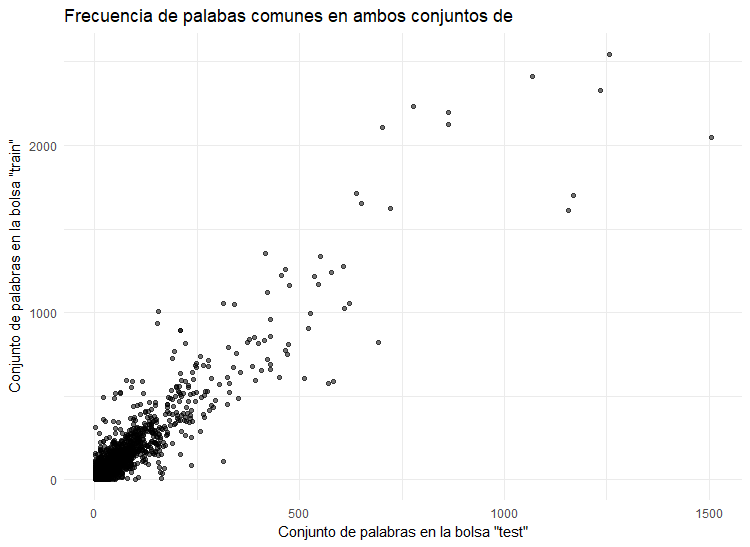
\includegraphics[scale=.6]{palabras1.png}
    \caption{Diagrama de dispersión de las palabras en común de los corpus ‘training’ y ‘test’ nótese que existe correlación positiva, este conjunto de palabras se utilizó en el análisis. ($\rho=0.98$.)}
    \label{figura5_1}
  \end{center}
\end{figure}
\FloatBarrier

\begin{enumerate}
\item \textit{Implementa clasicadores de Spam usando regresion logística, \textbf{LDA, QDA, FDA, Kernel FDA} y redes neuronales. Usa los datos \textbf{email\_train} e \textbf{email\_test} para ajustar y probar los métodos, respectvamente. Compara su desempeño.}\\

Como este inciso consiste en comparar el desempeño de diferentes algoritmos sobre un mismo conjunto de datos y el siguiente inciso lo aborda con más detalle, y considerando los comentarios respecto a la búsqueda de parámetros adecuados para un modelo dado ( discutido y experimentado en el ejercicio anterior). En este inciso me restrinjo a utilizar los métodos implementados en este tarea y en los que no lo fueron hago uso de diversos packages del entorno R, a continuación detallo los parámetros utilizados en cada implementación (cuando no se usaron los valores por default) podría pensarse que existe un sesgo en los resultados pues solo KLDA tiene parámetros que fueron ardua mente elegidos sin embargo la implementación de KLDA se restringe a un solo kernel lo que lo disminuye esta brecha.\\

Para el algoritmo de regresión logística utilice el package ‘glmnet’ desarrollado por el uno de los autores de \cite{Hes}. El método ‘glmnet’ en particular resuelve el problema de regresión logística sin embargo utiliza una función objetivo para la regresión logística penalizada utilizando la verosimilitud de la distribución binomial negativa (como puede verificarse en su respectiva vignette) \footnote{La cual me parece una de las vignettes más ilustrativas del entorno R, como comentario personal la leí hace un par de años y me pareció complicada y el día de hoy me parece muy útil} sin embargo con fijar los parámetros $\lambda $ y $\alpha$ a cero (que se puede consultar en la ayuda de R) tenemos el modelo que  abordamos en clase.\\ Para las implementaciones de los clasificadores LDA y QDA utilice los implementados en el clásico package ‘MASS’ . Para aplicar KFLDA utilice mi implementación con los “mejores” parámetros encontrados en el ejercicio 4 al igual que el FDA que implementamos en el ejercicio 2 y finalmente para la red neuronal decidí utilizar un package con más tiempo en los repositorios de CRAN, el package ‘nnet’ \footnote{Pues también hace un par de años lo utilice y me pareció poco sencillo de utilizar} en vista de que su objetivo es más acotado y se asemeja más al modelo de perceptrón que vimos en clase\footnote{En este caso la elección de parámetros se concentró en las sugerencias que ya he mencionado en el ejercicio 3 que se pueden encontrar en \cite{Hes}}. Los resultados de accuracy de los diversos algoritmos se reportan en el cuadro 5.1 donde se encuentran los resultados para diversos valores de $n$ número de palabras. (es decir la dimensionalidad del problema).\footnote{Los asteriscos señalan que la implementación no logro efectuar la estimación}\\  
\[\]
\begin{minipage}{\linewidth}
\centering
\begin{tabular}{|l|c|c|c|c|c|}\hline
Algoritmo           &  $n=8 $ & $n=42$ & $n=101$ & $n=259$ &  $n=2154$ \\ \hline
Regresión logística &71\% 	 &     76\%  &    81.3\% & .77\%     &.72\% \\
LDA                & 63\%	 &    75\%   & 79\%      & 77\%      &54\%\\
QDA 			  & 69\%	&     72\%   &  77\%     & 74\%     &*  \\
FDA 			 & 50\% 	&    50\%   & 50\%       & 50\%    &  *\\
Kernel FDA 		& 50\%	   &     50\%  &  50\%      &50\%    & 50\%\\
Red neuronal 	& 	72\%	&    75\%  & 85\%       &82\%  & *\\ \hline
\end {tabular}
\captionof{table}{Accuracy reportado por diferentes algoritmos de clasificación efectuados sobre el conjunto de datos PIMA, se entrenaron con la partición ‘pima.tr’ y se validaron con la muestra ‘pima.te’ }
\label{comparacion_PIMA} 
\end{minipage}


Del cuadro 5.1 podemos deducir que la red neuronal en general funciona mejor para la tarea de clasificar, sin embargo, la aumentar la dimensionalidad pierde este lugar de favorito, seguido de el esta la tradicional regresión logística. Cabe mencionar en general el tiempo de ejecución de la red neuronal es casi el doble al de la regresión logística. Comprobamos con tristeza que las dos implementaciones realizadas en los ejercicios anteriores FDA y Kernel FDA se desempeñaron pobremente, pero esto se debe a que fijamos los parámetros de las experiencias anteriores.\\

\item \textit{Las curvas ROC (Receiver Operating Characteristics) es un método muy común para comparar algoritmos de clasicación binarios basado en la tabla de errores (falsos positivos y falsos negativos) que se cometen. Usa los resultados del inciso anterior para comparar los clasicadores usando este criterio. ¿ Cuál método elegirias? Usa el criterio del area bajo la curva (AUC).}


\begin{figure}[H]
  \begin{center}
    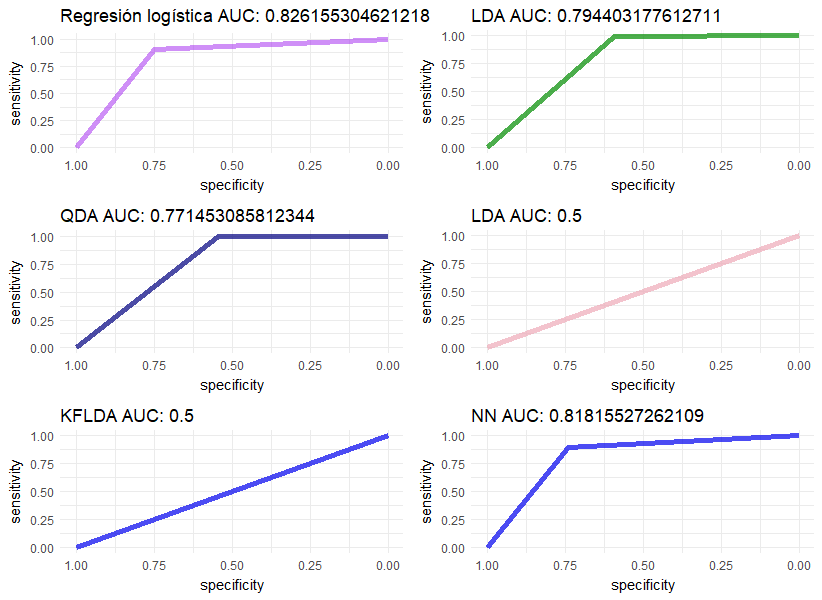
\includegraphics[scale=.6]{rocs.png}
    \caption{Curvas ROC para los algoritmos de clasificación del cuadro 5.1, fijando a 100 el numero de palabras con mayor frecuencia en el corpus de emails.}
    \label{figura5_2}
  \end{center}
\end{figure}
\FloatBarrier
Del cuadro 5.1 podriamos inferir que 100 palabras de todo el conjunto de palabras que construimos bastan para clasificar muy probablemente un correo como ‘spam’ o ‘no-spam’. Fijamos ese número de palabras y obtenemos sus curvas ROC para todos los modelos de la tabla, la serie de curvas se encuentra en la figura 5.2, es notar el pobre rendimiento de nuestras implementaciones (debido a que los parámetros se fijaron en función de otra muestra, de hecho, otro conjunto de datos totalmente diferente). Igualmente en la figura 5.2 es notable que bajo el criterio de área bajo la curva de ROC (AUC) las redes neuronales perfilan por debajo de la regresión lineal e inclusive su tiempo de ejecución es mucho mayor, por lo que para un problema de clasificación binario preferiría utilizar a la regresión logística en vista de este ejercicio y reafirmando la frase al final del capitulo de separadores lineales de \cite{Has}. 
\end{enumerate}



\begin{thebibliography}{1}
\bibitem{Hes}
Hastie T., Tibshirani R. and Friedman J. , \textit{The Elements of Statistical Larning}, Springer 2nd., 2009.

\end{thebibliography}

\end{document}